\documentclass[12pt]{article}

\usepackage{amsmath}

\fontfamily{lmss}
\usepackage{fullpage}
\usepackage{amsmath}
\usepackage{amsthm}
\usepackage{url}
\usepackage{multicol}
\usepackage{enumerate}
\usepackage{graphicx}
\usepackage{color}

\usepackage{xcolor}

\usepackage{tikz}
\usetikzlibrary{graphs}
\usetikzlibrary{arrows.meta,shapes,shapes.geometric}
\usetikzlibrary{positioning, quotes}

\tikzset{
  % Two node styles for game trees: solid and hollow
  solid node/.style={circle,draw,inner sep=1.2,fill=black},
  hollow node/.style={circle,draw,inner sep=1.2},
  % styles for long branch labels
  left label/.style={above left,midway},
  right label/.style={above right,midway}
}

\usepackage{hyperref}
\hypersetup{
    colorlinks=true,
    linkcolor=blue,
    filecolor=magenta,      
    urlcolor=blue,
}

\usepackage{geometry}
\geometry{
  top=1in,            % <-- you want to adjust this
  bottom=1in,
  left=1in,
  right=1in,
  headheight=3ex,       % <-- and this
  headsep=4ex,          % <-- and this
}

\usepackage{lastpage}
\usepackage{fancyhdr}
\pagestyle{fancy}
\fancyhf{}
\renewcommand{\footrulewidth}{0.4pt}
\lhead{CS 486/686}
\rfoot{Page \thepage\ of \pageref{LastPage}}

\setlength{\parskip}{\baselineskip}%
\setlength{\parindent}{0pt}%

\usepackage{tcolorbox}
\tcbuselibrary{breakable}
\newenvironment{markscheme}
{
    \renewcommand{\parskip}{\baselineskip}
    \begin{tcolorbox}[
        colback=blue!10,
        colframe=blue!10,
        sharp corners,
        breakable
    ]
    \textbf{Marking Scheme:}
}
{
    \end{tcolorbox}
}

\newenvironment{sol}
{
    \renewcommand{\parskip}{\baselineskip}
    \begin{tcolorbox}[
        colback=magenta!10,
        colframe=magenta!10,
        sharp corners,
        breakable
    ]
    \textbf{Solutions:}
}
{
    \end{tcolorbox}
}

\newenvironment{example}
{
    \renewcommand{\parskip}{\baselineskip}
    \begin{tcolorbox}[
        colback=green!10,
        colframe=green!10,
        sharp corners,
        breakable
    ]
}
{
    \end{tcolorbox}
}

\lhead{CS 486/686}
\chead{Winter 2022}
\rhead{Assignment 1}
\cfoot{v1.2}
\lfoot{\copyright Alice Gao \& Blake VanBerlo 2022}

\title{CS 486/686 Assignment 1 (122 marks) \\
}
\author{Blake VanBerlo}
\date{Due Date: 11:59 pm on Wednesday, February 2, 2021}

\hyphenation{PYTHONHASHSEED}

\begin{document}

\maketitle

\section*{Changes}

\begin{itemize}
\item v1.1: Marking scheme for Q1d
\item v1.2: Marking scheme for Q2c
\end{itemize}

\newpage
\section*{Academic Integrity Statement}

{\color{red} If your written submission on Learn does not include this academic integrity statement with your signature (typed name), we will deduct 5 marks from your final assignment mark.}

I declare the following statements to be true:

\begin{itemize}
\item 
The work I submit here is entirely my own.

\item 	
I have not shared and will not share any of my code with anyone at any point. 

\item 
I have not posted and will not post my code on any public or private forum or website.

\item 	
I have not discussed and will not discuss the contents of this assessment with anyone at any point.

\item 
I have not posted and will not post the contents of this assessment and its solutions on any public or private forum or website. 

\item 
I will not search for assessment solutions online.

\item 
I am aware that misconduct related to assessments can result in significant penalties, possibly including failure in the course and suspension. This is covered in Policy 71: https://uwaterloo.ca/secretariat/policies-procedures-guidelines/policy-71.
\end{itemize}

By typing or writing my full legal name below, I confirm that I have read and understood the academic integrity statement above.


\newpage
\section*{Instructions}

\begin{itemize}
\item
Submit any written solutions in a file named \verb+writeup.pdf+ to the A1 Dropbox on \verb+Learn+. {\color{red} If your written submission on Learn does not contain \textbf{one} file named \verb+writeup.pdf+, we will deduct 5 marks from your final assignment mark.} 
\item Submit any code to \verb+Marmoset+ at \url{https://marmoset.student.cs.uwaterloo.ca/}. 
No late assignment will be accepted. This assignment is to be done individually.

\item 
I strongly encourage you to complete your write-up in LaTeX, using this source file. If you do, in your submission, please replace the author with your name and student number. Please also remove the due date, the Instructions section, and the Learning goals section. Thanks!

\item
Lead TAs: 
\begin{itemize}
\item 
Blake Vanberlo (bvanberlo@uwaterloo.ca)
\item
Dake Zhang (dake.zhang@uwaterloo.ca)
\end{itemize}
The TAs' office hours will be posted on MS Teams.
\end{itemize}



\section*{Learning goals}

{\bf Uninformed and Heuristic Search}
\begin{itemize}
\item Formulate a given problem as a heuristic search problem. Define the states, the initial state, the goal states, the action, the successor function, and the cost function.
\item Trace the execution of Breadth-First Search and Depth-First Search.
\item Define an admissible heuristic by solving a relaxed problem optimally. Explain why a heuristic is admissible.
\item Trace the execution of the A* search algorithm with an admissible heuristic.
\item Implement the A* search algorithm.
\end{itemize}




\newpage
\section{Shortest Route to Waterloo (22 marks)}

Suppose that you want to drive to Waterloo from your family home in Toronto, since classes are returning to in-person delivery. You are conscious of your carbon footprint; therefore, you are seeking the shortest path from your house to Waterloo.

Below is a graph indicating the driving distances between various cities surrounding Toronto and Waterloo. All distances are given in kilometres.

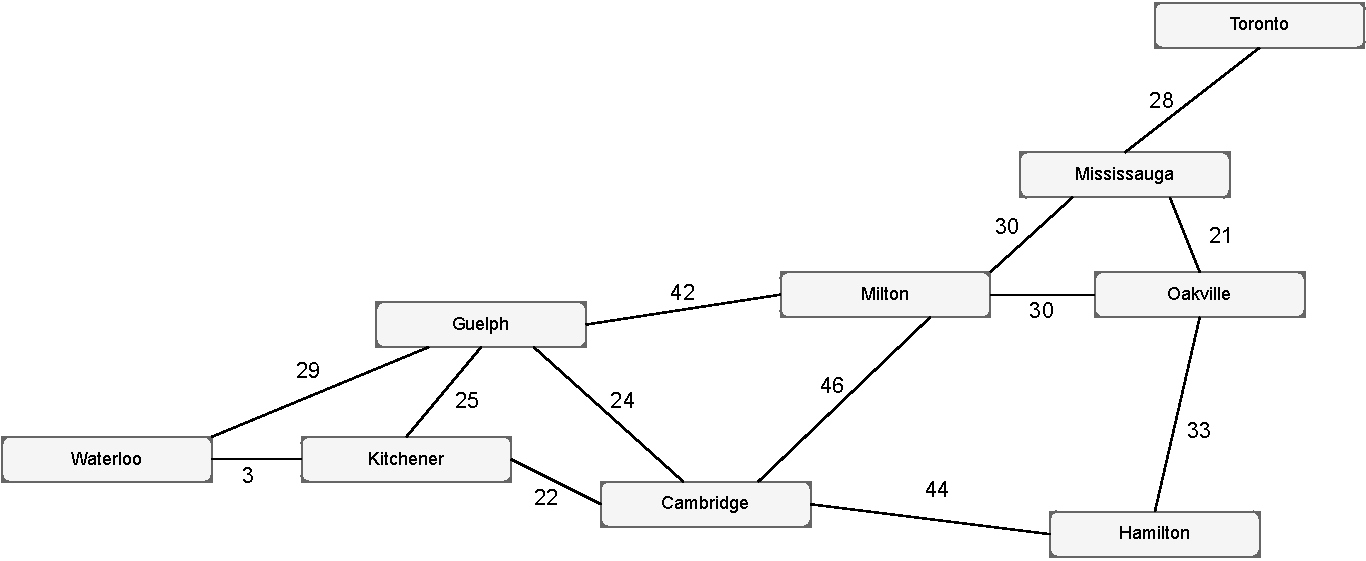
\includegraphics[width=\textwidth]{images_posted/Distance_map.pdf}

You would like to apply A* search to identify the shortest route to Waterloo from your house in Toronto. Below are the components of the search problem formulation:

\begin{itemize}
    \item \textbf{States:} Each city is the state. We will identify each state by the first 3 letters of its name. For example, the ``Guelph" node is denoted as \texttt{Gue}.
    \item \textbf{Initial state:} \texttt{Tor}
    \item \textbf{Goal state:} \texttt{Wat}
    \item \textbf{Successor function:} State B is a successor of state A if and only if there exists an edge on the above graph connecting city B and city A.
    \item \textbf{Cost function:} The cost of an edge connecting two states is the distance between the cities that the states correspond to.
\end{itemize}


Your decide to use Euclidean distance as a heuristic function. That is, $h$ is the Euclidean distance from a city to Waterloo (in kilometres). That is, if $(x_C,y_C)$ is city $C$'s longitude and latitude coordinates, $h(C) = \sqrt{(x_C - x_{Wat})^2 + (y_C - y_{Wat})^2}$. On the diagram below, the red text number to each city indicates its Euclidean distance to Waterloo.

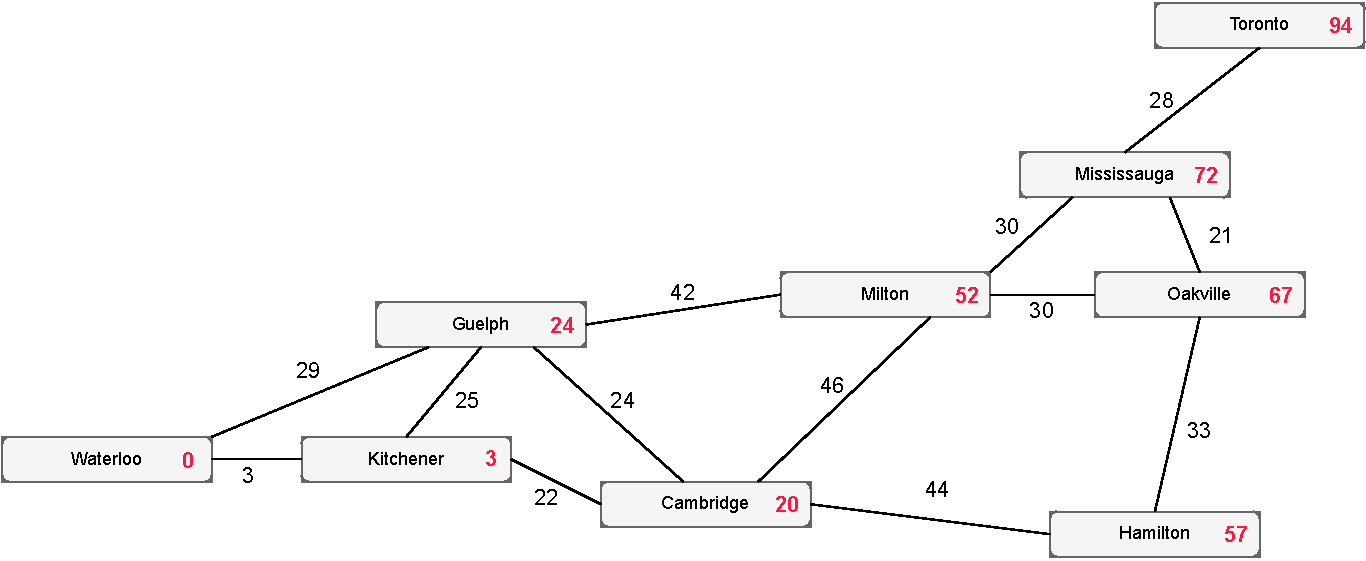
\includegraphics[width=\textwidth]{images_posted/Heuristic_map.pdf}



{\bf Please complete the following tasks.}

\begin{enumerate}[(a)]


%%%%%%%%%%%%%%%%%%%%%%%%%%%%%%%%%%%%%%%%%%%%%%%%%%%%%%
%%% Heuristic Function
%%%%%%%%%%%%%%%%%%%%%%%%%%%%%%%%%%%%%%%%%%%%%%%%%%%%%%
\item
\label{heuristic}
In no more than one paragraph, describe why the Euclidean distance to the destination is an admissible heuristic function.

\begin{markscheme}
(4 marks)

\begin{itemize}
\item
(4 marks) A reasonable explanation
\end{itemize}

\end{markscheme}

\item
\label{heuristic}
In no more than one paragraph, describe why Euclidean distance to the destination is a consistent heuristic function.

\begin{markscheme}
(4 marks)

\begin{itemize}
\item
(4 marks) A reasonable explanation
\end{itemize}

\end{markscheme}

\item
\label{heuristic}
Prove that a heuristic function that is consistent is also admissible.

Hint: try a direct proof. Apply the definition of a consistent heuristic across an optimal path from some arbitrary node to a goal.  %proof by contradiction. Assume that $h$ is a consistent heuristic function that is \textit{not} admissible.

\begin{markscheme}
(6 marks)

\begin{itemize}
\item
(4 marks) Correct proof
\item
(2 marks) The proof is clear, succinct, and easy to understand
\end{itemize}

\end{markscheme}

%%%%%%%%%%%%%%%%%%%%%%%%%%%%%%%%%%%%%%%%%%%%%%%%%%%%%%
%%% Execute the A* Search Algorithm
%%%%%%%%%%%%%%%%%%%%%%%%%%%%%%%%%%%%%%%%%%%%%%%%%%%%%%

\item
\label{execute_a_star}
Execute the A* search algorithm on the problem using the Euclidean distance heuristic function as described above. Do not perform any pruning. Add nodes to the frontier in alphabetical order. Remember to stop if you expand the goal state.

When drawing nodes, remember to abbreviate cities by writing the first 3 letters. For example, label a ``Waterloo" node as \texttt{Wat}. Annotate each node in the following format: $C + H = F$ where $C$ is the cost of the path, $H$ is the heuristic value, and $F$ is the sum of the cost and the heuristic values. Clearly indicate which nodes you expanded and in what order. You do not need to write out the frontier, but the tree must show all paths expanded after removing a node from the frontier.

Break any $F$-value ties using alphabetical order. For example, ``Milton" precedes ``Mississauga" and should be expanded first if the $F$ values for both nodes are the same.

We recommend using \url{https://app.diagrams.net/} to draw the search tree.

\begin{markscheme}
(8 marks) Correct search tree with all nodes correctly expanded in order.
\end{markscheme}


\end{enumerate}



\newpage
\section{The Rush Hour Sliding Puzzle (100 marks)}

In this programming question, you will solve the Rush Hour puzzle using the A* search and the depth-first search algorithms.

Take a look at an example of a Rush Hour puzzle below. The puzzle is on a 6 by 6 grid. We will number the rows as 0 to 5 from the top, and the columns as 0 to 5 from the left. In row 2, a horizontal car of length 2, called the goal car, is trying to escape through the exit on the right. There are horizontal and vertical cars of various lengths in the grid. A horizontal car can only move horizontally, whereas a vertical car can only move vertically. Each car may move more than one square in one step, but it cannot move over or through other cars. The goal is to move the cars around until the goal car reaches the exit, i.e. until the goal car is in the columns 4 and 5 in row 2. 

\begin{figure}[ht]
\centering
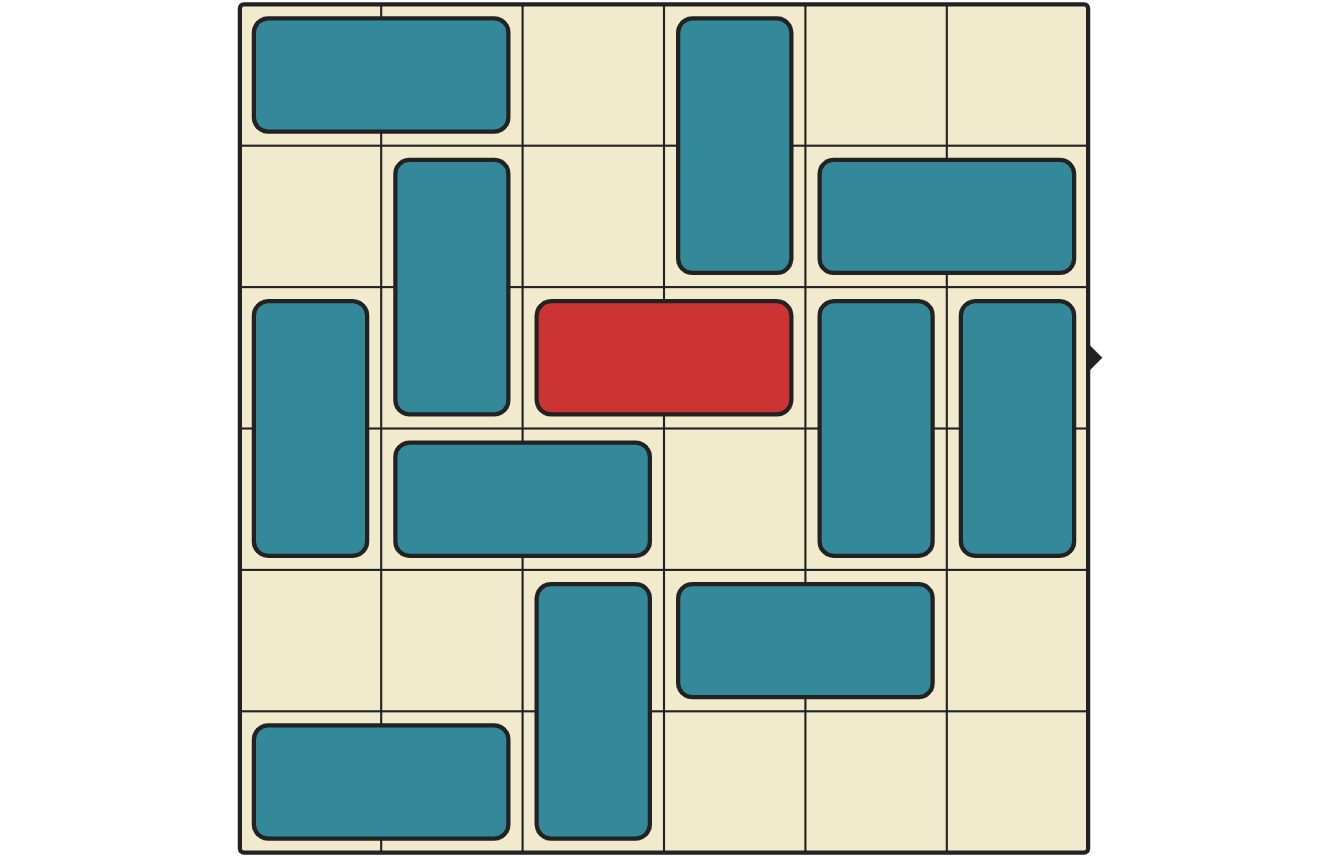
\includegraphics[width=0.7\textwidth]{images_posted/rush_hour_example.png}
\caption{An example of a Rush Hour puzzle from https://www.michaelfogleman.com/rush/}
\label{rush_hour_example}
\end{figure}

You can make the following assumptions for this question.
\begin{itemize}
  \item The puzzle must be on a 6 x 6 grid.
  \item The goal car is in row 2 and it has a length of 2.
  \item Besides the goal car, there is no other horizontal car in row 2.
\end{itemize}

{\bf Information on the Provided Code}

We have provided three files \verb+board.py+,  \verb+solve.py+, and \verb+jams_posted.txt+ on Learn. \verb+board.py+ contains code for handling input/output, representing states, etc. Your main task is to fill in the empty functions in \verb+solve.py+.

Submit the \verb+solve.py+ to Marmoset only. We will use our version of \verb+board.py+ to test your code. Do not modify any provided function signatures in \verb+solve.py+. Doing so will cause you to fail our tests. Feel free to add any new code to \verb+solve.py+. 

{\bf Input Format}

The file \verb+jams_posted.txt+ contains $40$ puzzles. You can use these puzzles to test your program. We will test your program using a different set of puzzles.

Below is an example of an input describing a puzzle.

\begin{verbatim}
example
6
1 2 h 2
2 0 v 2
4 0 h 2
3 1 v 3
4 1 v 2
4 3 h 2
.  
\end{verbatim}

\begin{itemize}
\item The first line assigns a name to the puzzle. In this case, the name is ``example.''
\item The next line specifies the size of the grid. We only use 6 by 6 grid. So this number is always 6.
\item The next line ``\verb+1 2 h 2+'' gives a description of the goal car.  The first two numbers $(1,2)$ gives the $(x,y)$ coordinates of the upper left corner of the car. The next letter ``h'' indicates that the car is horizontal (``v'' would indicate that the car is vertical). The last number ``2'' indicates that the car has size 2.
\item Each subsequent line, except the last line, describe a car in the puzzle, using the same format.
\item The last line consists of a single period, indicating the end of the puzzle. 
\end{itemize}

You can include multiple puzzles consecutively in the same file using the above format. 

{\bf The Heuristic Functions for A* Search:}

We have provided the implementation of the zero Heuristic function, which assigns a heuristic value of 0 to every state.

You must implement two other heuristic functions for A* search.
\begin{itemize}

  \item \underline{Blocking Heuristic:} The heuristic value for any goal state is zero. For any non-goal state, the heuristic value is one plus the number of cars blocking the path to the exit. For example, for the state in Figure~\ref{rush_hour_example}, the blocking heuristic value is $3$.
  
  \item \underline{Advanced Heuristic:} Implement a third advanced heuristic of your choosing and invention. Your advanced heuristic should be consistent and should dominate the blocking heuristic.
  
\end{itemize}

{\bf Testing Your Program}

Debugging and testing are essential skills for computer scientists. For this question, debugging your program may be especially challenging because of ties. Among ``correct'' implementations, the number of nodes expanded may vary widely due to how we handle the nodes with the same heuristic value on the frontier. 

Please test your code using {\bf Python 3.8.5}. 

{\bf We rely on Python's hashing to generate a state's ID for breaking ties} (see the Breaking Ties section below). However, Python' hashing function is not deterministic across different sessions. For example, you may get different hashing values of the same object for running your program multiple times. {\bf Please set the environment variable PYTHONHASHSEED to 486 BEFORE running the Python script.} Note that setting the variable in the code/program will not work.

Implement {\bf multi-path pruning for both DFS and A*}. When there are multiple paths to a state, multi-path pruning explores the first path to the state and discards any subsequent path to the same state. Use an explored set to keep track of the states that have been expanded by the algorithm. When you {\bf remove} a state from the frontier, check whether the state is in the explored set or not. If the state is in the explored set, then do nothing. Otherwise, add the state to the explored set and continue with the algorithm. Note that we perform pruning after we {\bf remove} a state from the frontier, not before we {\bf add} a state to the frontier.

DFS's behaviour depends on the order of adding a state's successors to the frontier. We will break ties by using the states' ID values. At each step, DFS will add the successors to the frontier in {\bf decreasing} order of their IDs. In other words, DFS will expand the state with the smallest ID value among the successors.

A* search will also break ties using the states' ID values. Among several states with the same $f$ value, A* will expand the state with the smallest ID value. If two states have the same ID value, A* will break ties using the states' parents --- expanding the state whose parent has the smaller ID value.

{\bf Please complete the following tasks:}

Submit your solutions to part (a) on Marmoset and submit your solutions to parts (b) and (c) on Learn.

\begin{enumerate}[(a)]

\item Complete the empty functions in \verb+solve.py+ and submit \verb+solve.py+ on \href{https://marmoset.student.cs.uwaterloo.ca/}{Marmoset}. Marmoset will evaluate your program for its correctness and efficiency.

For correctness, we have written unit tests for these functions: \verb+get_path+, \verb+is_goal+, \verb+blocking_heuristic+, \verb+get_successors+, \verb+dfs+, \verb+a_star+.

For each function, Marmoset provides one public test, which tests the function in a trivial scenario. There are also several secret tests. Before the deadline, you can only view the results of the public tests. After the deadline, Marmoset will run all the tests and calculate your marks.

Each test runs the function up to a predefined time limit. If the test passes if and only if the function terminates within the time limit and returns the expected result. Each test is all or nothing --- there are no partial marks available.

\begin{markscheme}
(88 marks) 

Unit tests on \verb+get_path+, \verb+is_goal+, \verb+blocking_heuristic+, \verb+get_successors+, \verb+dfs+, and \verb+a_star+. 

\begin{itemize}
\item \verb+get_path+: (1 public test + 2 secret tests) * 1 mark = 3 marks.
\item \verb+is_goal+:  (1 public test + 4 secret tests) * 1 mark = 5 marks.
\item \verb+blocking_heuristic+: (1 public test + 9 secret tests) * 2 marks = 20 marks.
\item \verb+get_successors+: (1 public test + 9 secret tests) * 2 marks = 20 marks.
\item \verb+dfs+:    (1 public test + 9 secret tests) * 2 marks = 20 marks.
\item \verb+a_star+: (1 public test + 9 secret tests) * 2 marks = 20 marks.
\end{itemize}

\end{markscheme}
  
\item Prove that the blocking heuristic is consistent using the definition of a consistent heuristic. 
\begin{markscheme}
(4 marks) Proof is correct and easy to understand. 
\end{markscheme}
 
\item
Design and implement an advanced heuristic of your own invention. Your advanced heuristic should be consistent and dominate the blocking heuristic.

Describe your advanced heuristic \textit{in 6 sentences or less}.

Prove that your advanced heuristic dominates the provided heuristic. Be as succinct as possible.

Implement your advanced heuristic. Show program output to support that A* search with the advanced heuristic expands fewer nodes than A* search with the blocking heuristic on all the 40 provided puzzles. (Make sure that you use the same PYTHONHASHSEED for all the program runs.)

\begin{markscheme}
(8 marks)

\begin{itemize}
\item (3 marks) Heuristic description is clear and is no more than 6 sentences.
\item (3 marks) Correct proof. Proof is clear and succinct.
\item (2 marks) Program output supports that the advanced heuristic dominates the blocking heuristic. 
\end{itemize}

\end{markscheme}

\end{enumerate}



\end{document}





























